\scanpage{2}

\uline{Programme de travail}
\margin{\unsure{7|?}}

\uline{\unsure{A}}

\uline{Th. 1} $N(\unsure{\xi|\zeta})\subset\operatorname{Alb}(S)$ n'est autre\deleted{\unsure{des|donc}}\inserted{\figure{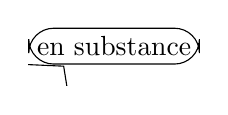
\begin{tikzpicture}\node[draw,rounded corners=9pt,inner sep=3pt](n){en substance};\draw(n.south west)--++(.45,-.02)--++(.04,-.25);\end{tikzpicture}}} que le noyau de l'application naturelle
\diagram{\begin{tikzcd}[ampersand replacement=\&]
\varphi_\xi:\operatorname{Alb}(S)\arrow[r]\&\unsure{\mathcal{Z}|Z}^{i}(X)/\unsure{\mathcal{Z}|Z}^{i}_{\mathrm{\unsure{alb|ab}}}(X)
\end{tikzcd}}
\margin{\figure{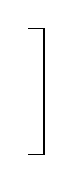
\begin{tikzpicture}\draw (0,0)--(.2,0)--(.2,1.6)--(0,1.6);\end{tikzpicture}}}

Th. 2 La dimension de $\operatorname{Alb}(S)/N(\xi)=P_\xi$ est majorée par un nb ne dépendant que de $X$ [en fait, par $\frac12 b^{2i-1}(X)$ !]
\margin{\figure{\begin{tikzpicture}\draw (0,0)--(.25,0)--(.25,1.9)--(0,1.9);\draw(.12,.85)--(.25,.85);\end{tikzpicture}}}

Ces deux th. impliquent

\uline{Th. 3}
$Z^i_{\mathrm{alg}}(X)/\unsure{\mathcal{Z}|Z}^{i}_{\mathrm{\unsure{alb|ab}}}(X)=\unsure{P}^{i}(X)$ a une structure naturelle de V.A., et $P^i(X)$ et $P^{\unsure{n-i|n+1-i}}(X)$ sont en dualité canonique.
\margin{\figure{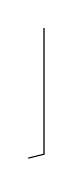
\begin{tikzpicture}\draw (0,0)--(.2,.05)--(.2,1.65);\end{tikzpicture}}}

\margin{\figure{\begin{tikzpicture}\node[draw,ellipse,align=center,inner sep=4pt](n){Connu\\tel\\quel};\draw[->](n.south east)--++(.35,-.2);\end{tikzpicture}}\uline{Hodge}}
\uline{Th. 4} Si $n=2m-1$, alors l'autodualité canonique de $P^m(X)$ [\unsure{donc la corr. sur} $\uline{P}^{m}(X)$] est \unsure{associé|associée} à une \uline{polarisation} de $P^m(X)$

\mspage{1}
